% Created by tikzDevice version 0.9 on 2016-01-11 22:38:33
% !TEX encoding = UTF-8 Unicode
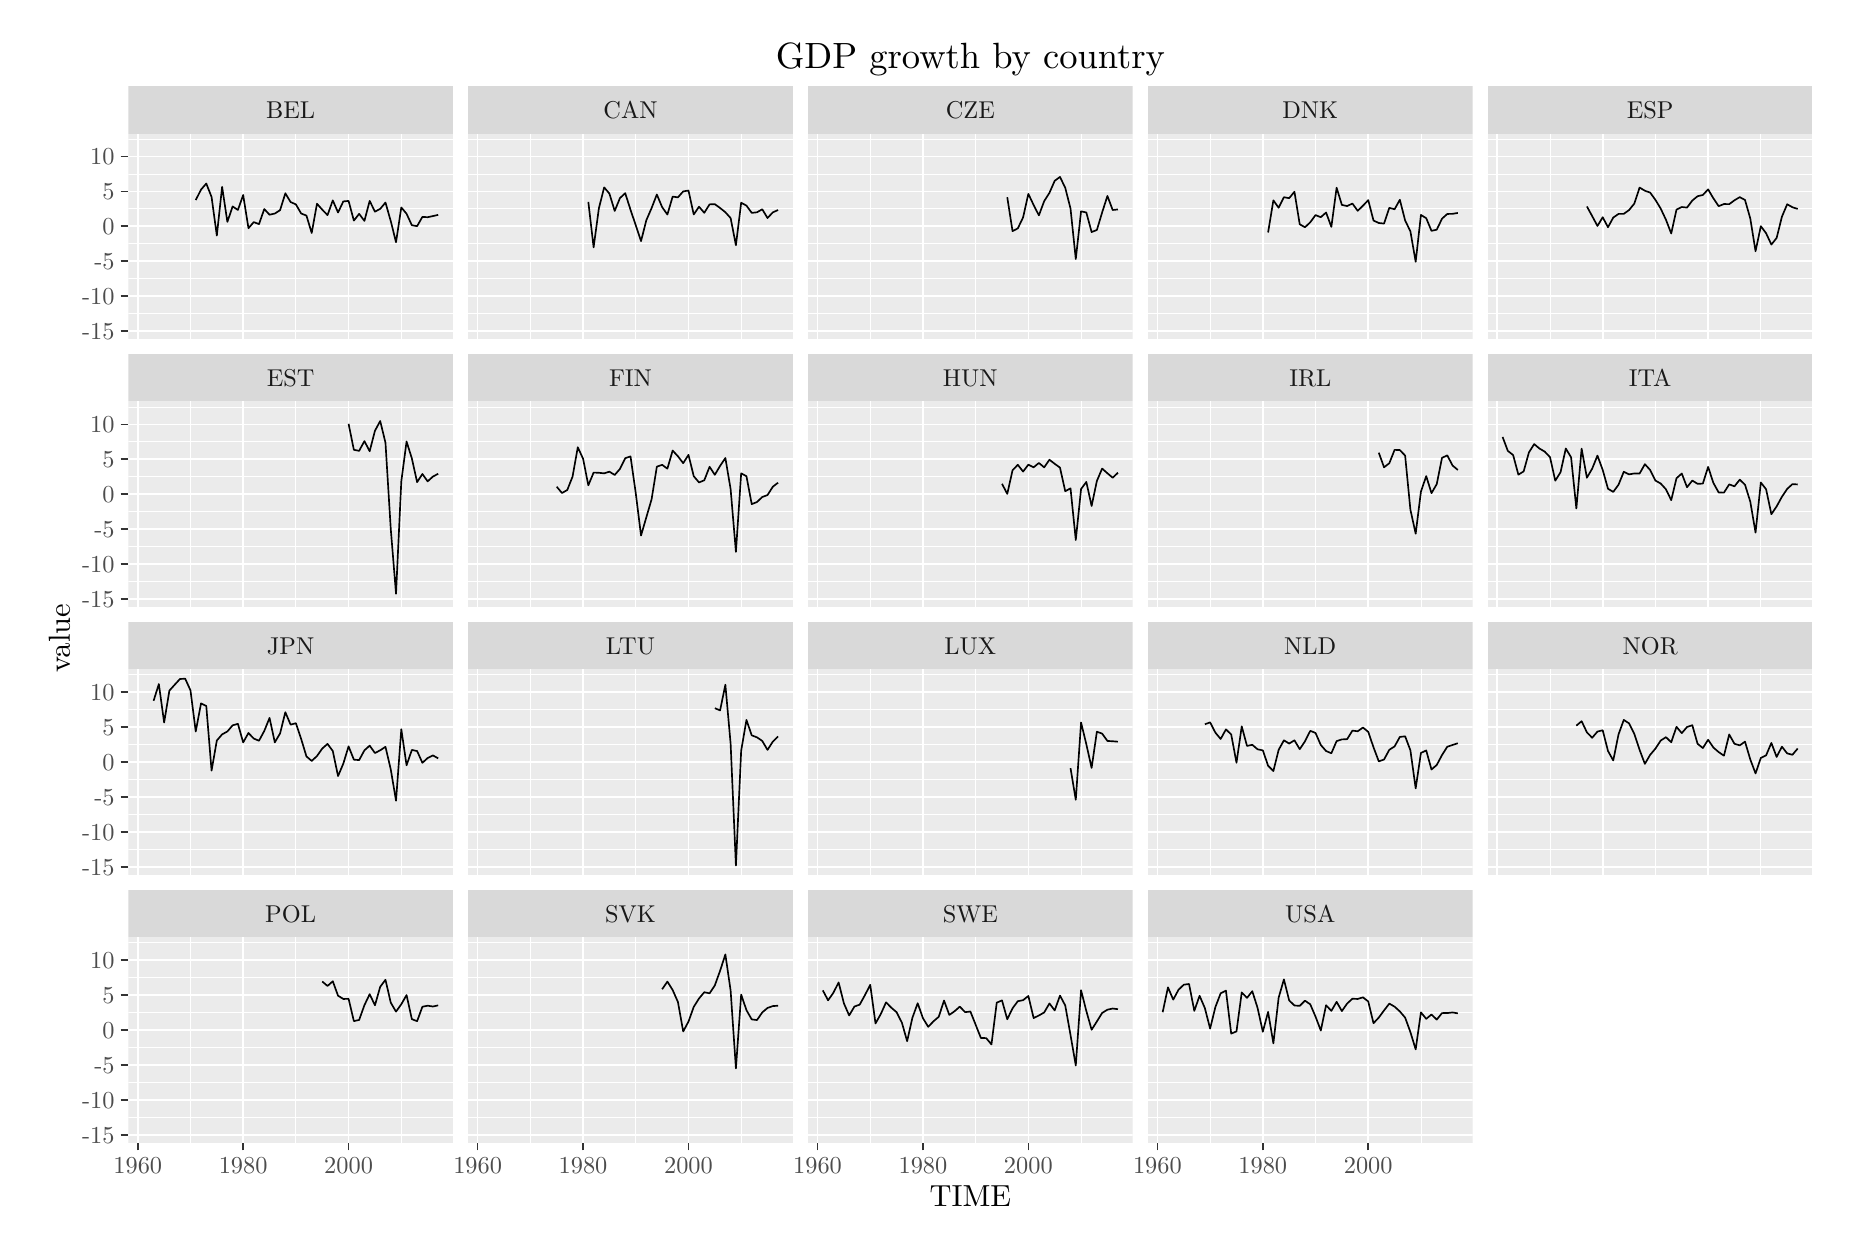
\begin{tikzpicture}[x=1pt,y=1pt]
\definecolor{fillColor}{RGB}{255,255,255}
\path[use as bounding box,fill=fillColor,fill opacity=0.00] (0,0) rectangle (650.43,433.62);
\begin{scope}
\path[clip] (  0.00,  0.00) rectangle (650.43,433.62);
\definecolor{drawColor}{RGB}{255,255,255}
\definecolor{fillColor}{RGB}{255,255,255}

\path[draw=drawColor,line width= 0.6pt,line join=round,line cap=round,fill=fillColor] (  0.00,  0.00) rectangle (650.43,433.62);
\end{scope}
\begin{scope}
\path[clip] ( 36.36,321.12) rectangle (153.67,395.37);
\definecolor{fillColor}{gray}{0.92}

\path[fill=fillColor] ( 36.36,321.12) rectangle (153.67,395.37);
\definecolor{drawColor}{RGB}{255,255,255}

\path[draw=drawColor,line width= 0.3pt,line join=round] ( 36.36,330.33) --
	(153.67,330.33);

\path[draw=drawColor,line width= 0.3pt,line join=round] ( 36.36,342.94) --
	(153.67,342.94);

\path[draw=drawColor,line width= 0.3pt,line join=round] ( 36.36,355.55) --
	(153.67,355.55);

\path[draw=drawColor,line width= 0.3pt,line join=round] ( 36.36,368.15) --
	(153.67,368.15);

\path[draw=drawColor,line width= 0.3pt,line join=round] ( 36.36,380.76) --
	(153.67,380.76);

\path[draw=drawColor,line width= 0.3pt,line join=round] ( 36.36,393.37) --
	(153.67,393.37);

\path[draw=drawColor,line width= 0.3pt,line join=round] ( 58.83,321.12) --
	( 58.83,395.37);

\path[draw=drawColor,line width= 0.3pt,line join=round] ( 96.92,321.12) --
	( 96.92,395.37);

\path[draw=drawColor,line width= 0.3pt,line join=round] (135.01,321.12) --
	(135.01,395.37);

\path[draw=drawColor,line width= 0.6pt,line join=round] ( 36.36,324.02) --
	(153.67,324.02);

\path[draw=drawColor,line width= 0.6pt,line join=round] ( 36.36,336.63) --
	(153.67,336.63);

\path[draw=drawColor,line width= 0.6pt,line join=round] ( 36.36,349.24) --
	(153.67,349.24);

\path[draw=drawColor,line width= 0.6pt,line join=round] ( 36.36,361.85) --
	(153.67,361.85);

\path[draw=drawColor,line width= 0.6pt,line join=round] ( 36.36,374.46) --
	(153.67,374.46);

\path[draw=drawColor,line width= 0.6pt,line join=round] ( 36.36,387.07) --
	(153.67,387.07);

\path[draw=drawColor,line width= 0.6pt,line join=round] ( 39.78,321.12) --
	( 39.78,395.37);

\path[draw=drawColor,line width= 0.6pt,line join=round] ( 77.87,321.12) --
	( 77.87,395.37);

\path[draw=drawColor,line width= 0.6pt,line join=round] (115.96,321.12) --
	(115.96,395.37);
\definecolor{drawColor}{RGB}{0,0,0}

\path[draw=drawColor,line width= 0.6pt,line join=round] ( 60.73,371.31) --
	( 62.64,375.10) --
	( 64.54,377.29) --
	( 66.45,372.44) --
	( 68.35,358.50) --
	( 70.26,376.11) --
	( 72.16,363.43) --
	( 74.06,369.02) --
	( 75.97,367.75) --
	( 77.87,373.15) --
	( 79.78,361.15) --
	( 81.68,363.35) --
	( 83.59,362.64) --
	( 85.49,368.07) --
	( 87.40,366.02) --
	( 89.30,366.45) --
	( 91.20,367.67) --
	( 93.11,373.76) --
	( 95.01,370.60) --
	( 96.92,369.76) --
	( 98.82,366.47) --
	(100.73,365.71) --
	(102.63,359.43) --
	(104.54,369.99) --
	(106.44,367.86) --
	(108.35,365.87) --
	(110.25,371.21) --
	(112.15,366.83) --
	(114.06,370.84) --
	(115.96,371.01) --
	(117.87,363.90) --
	(119.77,366.34) --
	(121.68,363.80) --
	(123.58,371.02) --
	(125.49,367.13) --
	(127.39,368.15) --
	(129.29,370.42) --
	(131.20,363.73) --
	(133.10,356.09) --
	(135.01,368.65) --
	(136.91,366.38) --
	(138.82,362.23) --
	(140.72,361.89) --
	(142.63,365.25) --
	(144.53,365.12) --
	(146.43,365.54) --
	(148.34,365.97);
\end{scope}
\begin{scope}
\path[clip] (159.17,321.12) rectangle (276.49,395.37);
\definecolor{fillColor}{gray}{0.92}

\path[fill=fillColor] (159.17,321.12) rectangle (276.49,395.37);
\definecolor{drawColor}{RGB}{255,255,255}

\path[draw=drawColor,line width= 0.3pt,line join=round] (159.17,330.33) --
	(276.49,330.33);

\path[draw=drawColor,line width= 0.3pt,line join=round] (159.17,342.94) --
	(276.49,342.94);

\path[draw=drawColor,line width= 0.3pt,line join=round] (159.17,355.55) --
	(276.49,355.55);

\path[draw=drawColor,line width= 0.3pt,line join=round] (159.17,368.15) --
	(276.49,368.15);

\path[draw=drawColor,line width= 0.3pt,line join=round] (159.17,380.76) --
	(276.49,380.76);

\path[draw=drawColor,line width= 0.3pt,line join=round] (159.17,393.37) --
	(276.49,393.37);

\path[draw=drawColor,line width= 0.3pt,line join=round] (181.64,321.12) --
	(181.64,395.37);

\path[draw=drawColor,line width= 0.3pt,line join=round] (219.73,321.12) --
	(219.73,395.37);

\path[draw=drawColor,line width= 0.3pt,line join=round] (257.82,321.12) --
	(257.82,395.37);

\path[draw=drawColor,line width= 0.6pt,line join=round] (159.17,324.02) --
	(276.49,324.02);

\path[draw=drawColor,line width= 0.6pt,line join=round] (159.17,336.63) --
	(276.49,336.63);

\path[draw=drawColor,line width= 0.6pt,line join=round] (159.17,349.24) --
	(276.49,349.24);

\path[draw=drawColor,line width= 0.6pt,line join=round] (159.17,361.85) --
	(276.49,361.85);

\path[draw=drawColor,line width= 0.6pt,line join=round] (159.17,374.46) --
	(276.49,374.46);

\path[draw=drawColor,line width= 0.6pt,line join=round] (159.17,387.07) --
	(276.49,387.07);

\path[draw=drawColor,line width= 0.6pt,line join=round] (162.60,321.12) --
	(162.60,395.37);

\path[draw=drawColor,line width= 0.6pt,line join=round] (200.69,321.12) --
	(200.69,395.37);

\path[draw=drawColor,line width= 0.6pt,line join=round] (238.78,321.12) --
	(238.78,395.37);
\definecolor{drawColor}{RGB}{0,0,0}

\path[draw=drawColor,line width= 0.6pt,line join=round] (202.59,370.68) --
	(204.50,354.23) --
	(206.40,368.32) --
	(208.31,375.90) --
	(210.21,373.65) --
	(212.12,367.39) --
	(214.02,372.04) --
	(215.92,373.80) --
	(217.83,367.84) --
	(219.73,362.18) --
	(221.64,356.50) --
	(223.54,364.01) --
	(225.45,368.43) --
	(227.35,373.33) --
	(229.26,368.76) --
	(231.16,366.09) --
	(233.06,372.58) --
	(234.97,372.29) --
	(236.87,374.45) --
	(238.78,374.77) --
	(240.68,366.11) --
	(242.59,368.92) --
	(244.49,366.71) --
	(246.40,369.77) --
	(248.30,369.83) --
	(250.20,368.46) --
	(252.11,366.92) --
	(254.01,364.81) --
	(255.92,355.01) --
	(257.82,370.36) --
	(259.73,369.32) --
	(261.63,366.70) --
	(263.54,366.90) --
	(265.44,368.00) --
	(267.34,364.82) --
	(269.25,366.88) --
	(271.15,367.72);
\end{scope}
\begin{scope}
\path[clip] (281.99,321.12) rectangle (399.30,395.37);
\definecolor{fillColor}{gray}{0.92}

\path[fill=fillColor] (281.99,321.12) rectangle (399.30,395.37);
\definecolor{drawColor}{RGB}{255,255,255}

\path[draw=drawColor,line width= 0.3pt,line join=round] (281.99,330.33) --
	(399.30,330.33);

\path[draw=drawColor,line width= 0.3pt,line join=round] (281.99,342.94) --
	(399.30,342.94);

\path[draw=drawColor,line width= 0.3pt,line join=round] (281.99,355.55) --
	(399.30,355.55);

\path[draw=drawColor,line width= 0.3pt,line join=round] (281.99,368.15) --
	(399.30,368.15);

\path[draw=drawColor,line width= 0.3pt,line join=round] (281.99,380.76) --
	(399.30,380.76);

\path[draw=drawColor,line width= 0.3pt,line join=round] (281.99,393.37) --
	(399.30,393.37);

\path[draw=drawColor,line width= 0.3pt,line join=round] (304.46,321.12) --
	(304.46,395.37);

\path[draw=drawColor,line width= 0.3pt,line join=round] (342.55,321.12) --
	(342.55,395.37);

\path[draw=drawColor,line width= 0.3pt,line join=round] (380.64,321.12) --
	(380.64,395.37);

\path[draw=drawColor,line width= 0.6pt,line join=round] (281.99,324.02) --
	(399.30,324.02);

\path[draw=drawColor,line width= 0.6pt,line join=round] (281.99,336.63) --
	(399.30,336.63);

\path[draw=drawColor,line width= 0.6pt,line join=round] (281.99,349.24) --
	(399.30,349.24);

\path[draw=drawColor,line width= 0.6pt,line join=round] (281.99,361.85) --
	(399.30,361.85);

\path[draw=drawColor,line width= 0.6pt,line join=round] (281.99,374.46) --
	(399.30,374.46);

\path[draw=drawColor,line width= 0.6pt,line join=round] (281.99,387.07) --
	(399.30,387.07);

\path[draw=drawColor,line width= 0.6pt,line join=round] (285.41,321.12) --
	(285.41,395.37);

\path[draw=drawColor,line width= 0.6pt,line join=round] (323.50,321.12) --
	(323.50,395.37);

\path[draw=drawColor,line width= 0.6pt,line join=round] (361.59,321.12) --
	(361.59,395.37);
\definecolor{drawColor}{RGB}{0,0,0}

\path[draw=drawColor,line width= 0.6pt,line join=round] (353.97,372.34) --
	(355.88,360.08) --
	(357.78,361.09) --
	(359.69,365.06) --
	(361.59,373.56) --
	(363.50,369.52) --
	(365.40,365.79) --
	(367.31,370.93) --
	(369.21,373.93) --
	(371.11,378.28) --
	(373.02,379.68) --
	(374.92,375.76) --
	(376.83,368.25) --
	(378.73,350.00) --
	(380.64,367.25) --
	(382.54,366.83) --
	(384.45,359.77) --
	(386.35,360.51) --
	(388.25,366.84) --
	(390.16,372.81) --
	(392.06,367.73) --
	(393.97,367.94);
\end{scope}
\begin{scope}
\path[clip] (404.80,321.12) rectangle (522.12,395.37);
\definecolor{fillColor}{gray}{0.92}

\path[fill=fillColor] (404.80,321.12) rectangle (522.12,395.37);
\definecolor{drawColor}{RGB}{255,255,255}

\path[draw=drawColor,line width= 0.3pt,line join=round] (404.80,330.33) --
	(522.12,330.33);

\path[draw=drawColor,line width= 0.3pt,line join=round] (404.80,342.94) --
	(522.12,342.94);

\path[draw=drawColor,line width= 0.3pt,line join=round] (404.80,355.55) --
	(522.12,355.55);

\path[draw=drawColor,line width= 0.3pt,line join=round] (404.80,368.15) --
	(522.12,368.15);

\path[draw=drawColor,line width= 0.3pt,line join=round] (404.80,380.76) --
	(522.12,380.76);

\path[draw=drawColor,line width= 0.3pt,line join=round] (404.80,393.37) --
	(522.12,393.37);

\path[draw=drawColor,line width= 0.3pt,line join=round] (427.27,321.12) --
	(427.27,395.37);

\path[draw=drawColor,line width= 0.3pt,line join=round] (465.36,321.12) --
	(465.36,395.37);

\path[draw=drawColor,line width= 0.3pt,line join=round] (503.45,321.12) --
	(503.45,395.37);

\path[draw=drawColor,line width= 0.6pt,line join=round] (404.80,324.02) --
	(522.12,324.02);

\path[draw=drawColor,line width= 0.6pt,line join=round] (404.80,336.63) --
	(522.12,336.63);

\path[draw=drawColor,line width= 0.6pt,line join=round] (404.80,349.24) --
	(522.12,349.24);

\path[draw=drawColor,line width= 0.6pt,line join=round] (404.80,361.85) --
	(522.12,361.85);

\path[draw=drawColor,line width= 0.6pt,line join=round] (404.80,374.46) --
	(522.12,374.46);

\path[draw=drawColor,line width= 0.6pt,line join=round] (404.80,387.07) --
	(522.12,387.07);

\path[draw=drawColor,line width= 0.6pt,line join=round] (408.23,321.12) --
	(408.23,395.37);

\path[draw=drawColor,line width= 0.6pt,line join=round] (446.32,321.12) --
	(446.32,395.37);

\path[draw=drawColor,line width= 0.6pt,line join=round] (484.41,321.12) --
	(484.41,395.37);
\definecolor{drawColor}{RGB}{0,0,0}

\path[draw=drawColor,line width= 0.6pt,line join=round] (448.22,359.61) --
	(450.13,371.22) --
	(452.03,368.54) --
	(453.94,372.36) --
	(455.84,372.00) --
	(457.74,374.33) --
	(459.65,362.58) --
	(461.55,361.49) --
	(463.46,363.30) --
	(465.36,365.90) --
	(467.27,365.13) --
	(469.17,366.83) --
	(471.08,361.62) --
	(472.98,375.78) --
	(474.88,369.58) --
	(476.79,369.16) --
	(478.69,370.07) --
	(480.60,367.44) --
	(482.50,369.28) --
	(484.41,371.30) --
	(486.31,363.93) --
	(488.22,363.03) --
	(490.12,362.83) --
	(492.02,368.51) --
	(493.93,368.00) --
	(495.83,371.43) --
	(497.74,363.93) --
	(499.64,360.04) --
	(501.55,349.02) --
	(503.45,365.95) --
	(505.36,364.76) --
	(507.26,360.20) --
	(509.16,360.62) --
	(511.07,364.60) --
	(512.97,366.30) --
	(514.88,366.35) --
	(516.78,366.67);
\end{scope}
\begin{scope}
\path[clip] (527.62,321.12) rectangle (644.93,395.37);
\definecolor{fillColor}{gray}{0.92}

\path[fill=fillColor] (527.62,321.12) rectangle (644.93,395.37);
\definecolor{drawColor}{RGB}{255,255,255}

\path[draw=drawColor,line width= 0.3pt,line join=round] (527.62,330.33) --
	(644.93,330.33);

\path[draw=drawColor,line width= 0.3pt,line join=round] (527.62,342.94) --
	(644.93,342.94);

\path[draw=drawColor,line width= 0.3pt,line join=round] (527.62,355.55) --
	(644.93,355.55);

\path[draw=drawColor,line width= 0.3pt,line join=round] (527.62,368.15) --
	(644.93,368.15);

\path[draw=drawColor,line width= 0.3pt,line join=round] (527.62,380.76) --
	(644.93,380.76);

\path[draw=drawColor,line width= 0.3pt,line join=round] (527.62,393.37) --
	(644.93,393.37);

\path[draw=drawColor,line width= 0.3pt,line join=round] (550.09,321.12) --
	(550.09,395.37);

\path[draw=drawColor,line width= 0.3pt,line join=round] (588.18,321.12) --
	(588.18,395.37);

\path[draw=drawColor,line width= 0.3pt,line join=round] (626.27,321.12) --
	(626.27,395.37);

\path[draw=drawColor,line width= 0.6pt,line join=round] (527.62,324.02) --
	(644.93,324.02);

\path[draw=drawColor,line width= 0.6pt,line join=round] (527.62,336.63) --
	(644.93,336.63);

\path[draw=drawColor,line width= 0.6pt,line join=round] (527.62,349.24) --
	(644.93,349.24);

\path[draw=drawColor,line width= 0.6pt,line join=round] (527.62,361.85) --
	(644.93,361.85);

\path[draw=drawColor,line width= 0.6pt,line join=round] (527.62,374.46) --
	(644.93,374.46);

\path[draw=drawColor,line width= 0.6pt,line join=round] (527.62,387.07) --
	(644.93,387.07);

\path[draw=drawColor,line width= 0.6pt,line join=round] (531.04,321.12) --
	(531.04,395.37);

\path[draw=drawColor,line width= 0.6pt,line join=round] (569.13,321.12) --
	(569.13,395.37);

\path[draw=drawColor,line width= 0.6pt,line join=round] (607.22,321.12) --
	(607.22,395.37);
\definecolor{drawColor}{RGB}{0,0,0}

\path[draw=drawColor,line width= 0.6pt,line join=round] (563.42,369.01) --
	(565.32,365.54) --
	(567.23,361.96) --
	(569.13,365.12) --
	(571.04,361.51) --
	(572.94,364.99) --
	(574.85,366.32) --
	(576.75,366.35) --
	(578.65,367.71) --
	(580.56,370.05) --
	(582.46,375.84) --
	(584.37,374.69) --
	(586.27,374.03) --
	(588.18,371.39) --
	(590.08,368.26) --
	(591.99,364.20) --
	(593.89,359.25) --
	(595.79,367.86) --
	(597.70,368.81) --
	(599.60,368.60) --
	(601.51,371.15) --
	(603.41,372.71) --
	(605.32,373.16) --
	(607.22,375.19) --
	(609.13,371.94) --
	(611.03,369.11) --
	(612.94,369.89) --
	(614.84,369.84) --
	(616.74,371.24) --
	(618.65,372.38) --
	(620.55,371.35) --
	(622.46,364.66) --
	(624.36,352.84) --
	(626.27,361.89) --
	(628.17,359.33) --
	(630.08,355.24) --
	(631.98,357.63) --
	(633.88,365.28) --
	(635.79,369.81) --
	(637.69,368.73) --
	(639.60,368.12);
\end{scope}
\begin{scope}
\path[clip] ( 36.36,224.31) rectangle (153.67,298.56);
\definecolor{fillColor}{gray}{0.92}

\path[fill=fillColor] ( 36.36,224.31) rectangle (153.67,298.56);
\definecolor{drawColor}{RGB}{255,255,255}

\path[draw=drawColor,line width= 0.3pt,line join=round] ( 36.36,233.52) --
	(153.67,233.52);

\path[draw=drawColor,line width= 0.3pt,line join=round] ( 36.36,246.13) --
	(153.67,246.13);

\path[draw=drawColor,line width= 0.3pt,line join=round] ( 36.36,258.74) --
	(153.67,258.74);

\path[draw=drawColor,line width= 0.3pt,line join=round] ( 36.36,271.34) --
	(153.67,271.34);

\path[draw=drawColor,line width= 0.3pt,line join=round] ( 36.36,283.95) --
	(153.67,283.95);

\path[draw=drawColor,line width= 0.3pt,line join=round] ( 36.36,296.56) --
	(153.67,296.56);

\path[draw=drawColor,line width= 0.3pt,line join=round] ( 58.83,224.31) --
	( 58.83,298.56);

\path[draw=drawColor,line width= 0.3pt,line join=round] ( 96.92,224.31) --
	( 96.92,298.56);

\path[draw=drawColor,line width= 0.3pt,line join=round] (135.01,224.31) --
	(135.01,298.56);

\path[draw=drawColor,line width= 0.6pt,line join=round] ( 36.36,227.21) --
	(153.67,227.21);

\path[draw=drawColor,line width= 0.6pt,line join=round] ( 36.36,239.82) --
	(153.67,239.82);

\path[draw=drawColor,line width= 0.6pt,line join=round] ( 36.36,252.43) --
	(153.67,252.43);

\path[draw=drawColor,line width= 0.6pt,line join=round] ( 36.36,265.04) --
	(153.67,265.04);

\path[draw=drawColor,line width= 0.6pt,line join=round] ( 36.36,277.65) --
	(153.67,277.65);

\path[draw=drawColor,line width= 0.6pt,line join=round] ( 36.36,290.26) --
	(153.67,290.26);

\path[draw=drawColor,line width= 0.6pt,line join=round] ( 39.78,224.31) --
	( 39.78,298.56);

\path[draw=drawColor,line width= 0.6pt,line join=round] ( 77.87,224.31) --
	( 77.87,298.56);

\path[draw=drawColor,line width= 0.6pt,line join=round] (115.96,224.31) --
	(115.96,298.56);
\definecolor{drawColor}{RGB}{0,0,0}

\path[draw=drawColor,line width= 0.6pt,line join=round] (115.96,290.47) --
	(117.87,281.07) --
	(119.77,280.71) --
	(121.68,284.22) --
	(123.58,280.57) --
	(125.49,287.96) --
	(127.39,291.48) --
	(129.29,283.62) --
	(131.20,252.50) --
	(133.10,229.08) --
	(135.01,269.68) --
	(136.91,284.06) --
	(138.82,277.98) --
	(140.72,269.39) --
	(142.63,272.34) --
	(144.53,269.67) --
	(146.43,271.41) --
	(148.34,272.42);
\end{scope}
\begin{scope}
\path[clip] (159.17,224.31) rectangle (276.49,298.56);
\definecolor{fillColor}{gray}{0.92}

\path[fill=fillColor] (159.17,224.31) rectangle (276.49,298.56);
\definecolor{drawColor}{RGB}{255,255,255}

\path[draw=drawColor,line width= 0.3pt,line join=round] (159.17,233.52) --
	(276.49,233.52);

\path[draw=drawColor,line width= 0.3pt,line join=round] (159.17,246.13) --
	(276.49,246.13);

\path[draw=drawColor,line width= 0.3pt,line join=round] (159.17,258.74) --
	(276.49,258.74);

\path[draw=drawColor,line width= 0.3pt,line join=round] (159.17,271.34) --
	(276.49,271.34);

\path[draw=drawColor,line width= 0.3pt,line join=round] (159.17,283.95) --
	(276.49,283.95);

\path[draw=drawColor,line width= 0.3pt,line join=round] (159.17,296.56) --
	(276.49,296.56);

\path[draw=drawColor,line width= 0.3pt,line join=round] (181.64,224.31) --
	(181.64,298.56);

\path[draw=drawColor,line width= 0.3pt,line join=round] (219.73,224.31) --
	(219.73,298.56);

\path[draw=drawColor,line width= 0.3pt,line join=round] (257.82,224.31) --
	(257.82,298.56);

\path[draw=drawColor,line width= 0.6pt,line join=round] (159.17,227.21) --
	(276.49,227.21);

\path[draw=drawColor,line width= 0.6pt,line join=round] (159.17,239.82) --
	(276.49,239.82);

\path[draw=drawColor,line width= 0.6pt,line join=round] (159.17,252.43) --
	(276.49,252.43);

\path[draw=drawColor,line width= 0.6pt,line join=round] (159.17,265.04) --
	(276.49,265.04);

\path[draw=drawColor,line width= 0.6pt,line join=round] (159.17,277.65) --
	(276.49,277.65);

\path[draw=drawColor,line width= 0.6pt,line join=round] (159.17,290.26) --
	(276.49,290.26);

\path[draw=drawColor,line width= 0.6pt,line join=round] (162.60,224.31) --
	(162.60,298.56);

\path[draw=drawColor,line width= 0.6pt,line join=round] (200.69,224.31) --
	(200.69,298.56);

\path[draw=drawColor,line width= 0.6pt,line join=round] (238.78,224.31) --
	(238.78,298.56);
\definecolor{drawColor}{RGB}{0,0,0}

\path[draw=drawColor,line width= 0.6pt,line join=round] (191.17,267.74) --
	(193.07,265.46) --
	(194.98,266.56) --
	(196.88,271.35) --
	(198.78,281.99) --
	(200.69,277.87) --
	(202.59,268.25) --
	(204.50,272.85) --
	(206.40,272.78) --
	(208.31,272.57) --
	(210.21,273.18) --
	(212.12,271.99) --
	(214.02,274.17) --
	(215.92,278.04) --
	(217.83,278.70) --
	(219.73,265.40) --
	(221.64,250.12) --
	(223.54,256.66) --
	(225.45,263.19) --
	(227.35,274.98) --
	(229.26,275.65) --
	(231.16,274.26) --
	(233.06,280.81) --
	(234.97,278.73) --
	(236.87,276.25) --
	(238.78,279.25) --
	(240.68,271.55) --
	(242.59,269.28) --
	(244.49,270.07) --
	(246.40,274.94) --
	(248.30,272.05) --
	(250.20,275.26) --
	(252.11,278.12) --
	(254.01,266.86) --
	(255.92,244.19) --
	(257.82,272.59) --
	(259.73,271.52) --
	(261.63,261.44) --
	(263.54,262.21) --
	(265.44,264.02) --
	(267.34,264.73) --
	(269.25,267.73) --
	(271.15,269.20);
\end{scope}
\begin{scope}
\path[clip] (281.99,224.31) rectangle (399.30,298.56);
\definecolor{fillColor}{gray}{0.92}

\path[fill=fillColor] (281.99,224.31) rectangle (399.30,298.56);
\definecolor{drawColor}{RGB}{255,255,255}

\path[draw=drawColor,line width= 0.3pt,line join=round] (281.99,233.52) --
	(399.30,233.52);

\path[draw=drawColor,line width= 0.3pt,line join=round] (281.99,246.13) --
	(399.30,246.13);

\path[draw=drawColor,line width= 0.3pt,line join=round] (281.99,258.74) --
	(399.30,258.74);

\path[draw=drawColor,line width= 0.3pt,line join=round] (281.99,271.34) --
	(399.30,271.34);

\path[draw=drawColor,line width= 0.3pt,line join=round] (281.99,283.95) --
	(399.30,283.95);

\path[draw=drawColor,line width= 0.3pt,line join=round] (281.99,296.56) --
	(399.30,296.56);

\path[draw=drawColor,line width= 0.3pt,line join=round] (304.46,224.31) --
	(304.46,298.56);

\path[draw=drawColor,line width= 0.3pt,line join=round] (342.55,224.31) --
	(342.55,298.56);

\path[draw=drawColor,line width= 0.3pt,line join=round] (380.64,224.31) --
	(380.64,298.56);

\path[draw=drawColor,line width= 0.6pt,line join=round] (281.99,227.21) --
	(399.30,227.21);

\path[draw=drawColor,line width= 0.6pt,line join=round] (281.99,239.82) --
	(399.30,239.82);

\path[draw=drawColor,line width= 0.6pt,line join=round] (281.99,252.43) --
	(399.30,252.43);

\path[draw=drawColor,line width= 0.6pt,line join=round] (281.99,265.04) --
	(399.30,265.04);

\path[draw=drawColor,line width= 0.6pt,line join=round] (281.99,277.65) --
	(399.30,277.65);

\path[draw=drawColor,line width= 0.6pt,line join=round] (281.99,290.26) --
	(399.30,290.26);

\path[draw=drawColor,line width= 0.6pt,line join=round] (285.41,224.31) --
	(285.41,298.56);

\path[draw=drawColor,line width= 0.6pt,line join=round] (323.50,224.31) --
	(323.50,298.56);

\path[draw=drawColor,line width= 0.6pt,line join=round] (361.59,224.31) --
	(361.59,298.56);
\definecolor{drawColor}{RGB}{0,0,0}

\path[draw=drawColor,line width= 0.6pt,line join=round] (352.07,268.80) --
	(353.97,265.15) --
	(355.88,273.68) --
	(357.78,275.66) --
	(359.69,273.22) --
	(361.59,275.70) --
	(363.50,274.75) --
	(365.40,276.34) --
	(367.31,274.73) --
	(369.21,277.49) --
	(371.11,276.02) --
	(373.02,274.64) --
	(374.92,266.11) --
	(376.83,267.16) --
	(378.73,248.50) --
	(380.64,266.91) --
	(382.54,269.47) --
	(384.45,260.78) --
	(386.35,269.81) --
	(388.25,274.30) --
	(390.16,272.60) --
	(392.06,271.00) --
	(393.97,272.80);
\end{scope}
\begin{scope}
\path[clip] (404.80,224.31) rectangle (522.12,298.56);
\definecolor{fillColor}{gray}{0.92}

\path[fill=fillColor] (404.80,224.31) rectangle (522.12,298.56);
\definecolor{drawColor}{RGB}{255,255,255}

\path[draw=drawColor,line width= 0.3pt,line join=round] (404.80,233.52) --
	(522.12,233.52);

\path[draw=drawColor,line width= 0.3pt,line join=round] (404.80,246.13) --
	(522.12,246.13);

\path[draw=drawColor,line width= 0.3pt,line join=round] (404.80,258.74) --
	(522.12,258.74);

\path[draw=drawColor,line width= 0.3pt,line join=round] (404.80,271.34) --
	(522.12,271.34);

\path[draw=drawColor,line width= 0.3pt,line join=round] (404.80,283.95) --
	(522.12,283.95);

\path[draw=drawColor,line width= 0.3pt,line join=round] (404.80,296.56) --
	(522.12,296.56);

\path[draw=drawColor,line width= 0.3pt,line join=round] (427.27,224.31) --
	(427.27,298.56);

\path[draw=drawColor,line width= 0.3pt,line join=round] (465.36,224.31) --
	(465.36,298.56);

\path[draw=drawColor,line width= 0.3pt,line join=round] (503.45,224.31) --
	(503.45,298.56);

\path[draw=drawColor,line width= 0.6pt,line join=round] (404.80,227.21) --
	(522.12,227.21);

\path[draw=drawColor,line width= 0.6pt,line join=round] (404.80,239.82) --
	(522.12,239.82);

\path[draw=drawColor,line width= 0.6pt,line join=round] (404.80,252.43) --
	(522.12,252.43);

\path[draw=drawColor,line width= 0.6pt,line join=round] (404.80,265.04) --
	(522.12,265.04);

\path[draw=drawColor,line width= 0.6pt,line join=round] (404.80,277.65) --
	(522.12,277.65);

\path[draw=drawColor,line width= 0.6pt,line join=round] (404.80,290.26) --
	(522.12,290.26);

\path[draw=drawColor,line width= 0.6pt,line join=round] (408.23,224.31) --
	(408.23,298.56);

\path[draw=drawColor,line width= 0.6pt,line join=round] (446.32,224.31) --
	(446.32,298.56);

\path[draw=drawColor,line width= 0.6pt,line join=round] (484.41,224.31) --
	(484.41,298.56);
\definecolor{drawColor}{RGB}{0,0,0}

\path[draw=drawColor,line width= 0.6pt,line join=round] (488.22,280.03) --
	(490.12,274.76) --
	(492.02,276.22) --
	(493.93,281.06) --
	(495.83,280.98) --
	(497.74,278.99) --
	(499.64,259.46) --
	(501.55,250.77) --
	(503.45,266.00) --
	(505.36,271.57) --
	(507.26,265.41) --
	(509.16,268.67) --
	(511.07,278.19) --
	(512.97,279.06) --
	(514.88,275.40) --
	(516.78,273.81);
\end{scope}
\begin{scope}
\path[clip] (527.62,224.31) rectangle (644.93,298.56);
\definecolor{fillColor}{gray}{0.92}

\path[fill=fillColor] (527.62,224.31) rectangle (644.93,298.56);
\definecolor{drawColor}{RGB}{255,255,255}

\path[draw=drawColor,line width= 0.3pt,line join=round] (527.62,233.52) --
	(644.93,233.52);

\path[draw=drawColor,line width= 0.3pt,line join=round] (527.62,246.13) --
	(644.93,246.13);

\path[draw=drawColor,line width= 0.3pt,line join=round] (527.62,258.74) --
	(644.93,258.74);

\path[draw=drawColor,line width= 0.3pt,line join=round] (527.62,271.34) --
	(644.93,271.34);

\path[draw=drawColor,line width= 0.3pt,line join=round] (527.62,283.95) --
	(644.93,283.95);

\path[draw=drawColor,line width= 0.3pt,line join=round] (527.62,296.56) --
	(644.93,296.56);

\path[draw=drawColor,line width= 0.3pt,line join=round] (550.09,224.31) --
	(550.09,298.56);

\path[draw=drawColor,line width= 0.3pt,line join=round] (588.18,224.31) --
	(588.18,298.56);

\path[draw=drawColor,line width= 0.3pt,line join=round] (626.27,224.31) --
	(626.27,298.56);

\path[draw=drawColor,line width= 0.6pt,line join=round] (527.62,227.21) --
	(644.93,227.21);

\path[draw=drawColor,line width= 0.6pt,line join=round] (527.62,239.82) --
	(644.93,239.82);

\path[draw=drawColor,line width= 0.6pt,line join=round] (527.62,252.43) --
	(644.93,252.43);

\path[draw=drawColor,line width= 0.6pt,line join=round] (527.62,265.04) --
	(644.93,265.04);

\path[draw=drawColor,line width= 0.6pt,line join=round] (527.62,277.65) --
	(644.93,277.65);

\path[draw=drawColor,line width= 0.6pt,line join=round] (527.62,290.26) --
	(644.93,290.26);

\path[draw=drawColor,line width= 0.6pt,line join=round] (531.04,224.31) --
	(531.04,298.56);

\path[draw=drawColor,line width= 0.6pt,line join=round] (569.13,224.31) --
	(569.13,298.56);

\path[draw=drawColor,line width= 0.6pt,line join=round] (607.22,224.31) --
	(607.22,298.56);
\definecolor{drawColor}{RGB}{0,0,0}

\path[draw=drawColor,line width= 0.6pt,line join=round] (532.95,285.73) --
	(534.85,280.69) --
	(536.76,279.19) --
	(538.66,272.09) --
	(540.57,273.28) --
	(542.47,280.13) --
	(544.37,283.14) --
	(546.28,281.54) --
	(548.18,280.42) --
	(550.09,278.43) --
	(551.99,269.92) --
	(553.90,272.99) --
	(555.80,281.55) --
	(557.71,278.35) --
	(559.61,259.87) --
	(561.51,281.50) --
	(563.42,270.99) --
	(565.32,274.25) --
	(567.23,278.99) --
	(569.13,273.81) --
	(571.04,267.01) --
	(572.94,265.86) --
	(574.85,268.48) --
	(576.75,273.14) --
	(578.65,272.20) --
	(580.56,272.53) --
	(582.46,272.50) --
	(584.37,275.88) --
	(586.27,273.80) --
	(588.18,269.96) --
	(590.08,268.90) --
	(591.99,266.80) --
	(593.89,262.88) --
	(595.79,270.79) --
	(597.70,272.51) --
	(599.60,267.56) --
	(601.51,269.97) --
	(603.41,268.79) --
	(605.32,268.87) --
	(607.22,274.91) --
	(609.13,269.10) --
	(611.03,265.67) --
	(612.94,265.60) --
	(614.84,268.59) --
	(616.74,267.88) --
	(618.65,270.29) --
	(620.55,268.46) --
	(622.46,262.35) --
	(624.36,251.16) --
	(626.27,269.28) --
	(628.17,266.82) --
	(630.08,257.82) --
	(631.98,260.62) --
	(633.88,264.09) --
	(635.79,266.95) --
	(637.69,268.68) --
	(639.60,268.56);
\end{scope}
\begin{scope}
\path[clip] ( 36.36,127.50) rectangle (153.67,201.75);
\definecolor{fillColor}{gray}{0.92}

\path[fill=fillColor] ( 36.36,127.50) rectangle (153.67,201.75);
\definecolor{drawColor}{RGB}{255,255,255}

\path[draw=drawColor,line width= 0.3pt,line join=round] ( 36.36,136.71) --
	(153.67,136.71);

\path[draw=drawColor,line width= 0.3pt,line join=round] ( 36.36,149.32) --
	(153.67,149.32);

\path[draw=drawColor,line width= 0.3pt,line join=round] ( 36.36,161.93) --
	(153.67,161.93);

\path[draw=drawColor,line width= 0.3pt,line join=round] ( 36.36,174.53) --
	(153.67,174.53);

\path[draw=drawColor,line width= 0.3pt,line join=round] ( 36.36,187.14) --
	(153.67,187.14);

\path[draw=drawColor,line width= 0.3pt,line join=round] ( 36.36,199.75) --
	(153.67,199.75);

\path[draw=drawColor,line width= 0.3pt,line join=round] ( 58.83,127.50) --
	( 58.83,201.75);

\path[draw=drawColor,line width= 0.3pt,line join=round] ( 96.92,127.50) --
	( 96.92,201.75);

\path[draw=drawColor,line width= 0.3pt,line join=round] (135.01,127.50) --
	(135.01,201.75);

\path[draw=drawColor,line width= 0.6pt,line join=round] ( 36.36,130.40) --
	(153.67,130.40);

\path[draw=drawColor,line width= 0.6pt,line join=round] ( 36.36,143.01) --
	(153.67,143.01);

\path[draw=drawColor,line width= 0.6pt,line join=round] ( 36.36,155.62) --
	(153.67,155.62);

\path[draw=drawColor,line width= 0.6pt,line join=round] ( 36.36,168.23) --
	(153.67,168.23);

\path[draw=drawColor,line width= 0.6pt,line join=round] ( 36.36,180.84) --
	(153.67,180.84);

\path[draw=drawColor,line width= 0.6pt,line join=round] ( 36.36,193.45) --
	(153.67,193.45);

\path[draw=drawColor,line width= 0.6pt,line join=round] ( 39.78,127.50) --
	( 39.78,201.75);

\path[draw=drawColor,line width= 0.6pt,line join=round] ( 77.87,127.50) --
	( 77.87,201.75);

\path[draw=drawColor,line width= 0.6pt,line join=round] (115.96,127.50) --
	(115.96,201.75);
\definecolor{drawColor}{RGB}{0,0,0}

\path[draw=drawColor,line width= 0.6pt,line join=round] ( 45.50,190.39) --
	( 47.40,196.44) --
	( 49.31,182.54) --
	( 51.21,194.07) --
	( 53.12,196.18) --
	( 55.02,198.26) --
	( 56.92,198.37) --
	( 58.83,194.16) --
	( 60.73,179.30) --
	( 62.64,189.45) --
	( 64.54,188.49) --
	( 66.45,165.14) --
	( 68.35,176.03) --
	( 70.26,178.25) --
	( 72.16,179.30) --
	( 74.06,181.52) --
	( 75.97,182.06) --
	( 77.87,175.33) --
	( 79.78,178.76) --
	( 81.68,176.74) --
	( 83.59,175.95) --
	( 85.49,179.49) --
	( 87.40,184.20) --
	( 89.30,175.37) --
	( 91.20,178.59) --
	( 93.11,186.25) --
	( 95.01,181.77) --
	( 96.92,182.28) --
	( 98.82,176.61) --
	(100.73,170.29) --
	(102.63,168.66) --
	(104.54,170.41) --
	(106.44,173.13) --
	(108.35,174.81) --
	(110.25,172.25) --
	(112.15,163.18) --
	(114.06,167.70) --
	(115.96,173.93) --
	(117.87,169.12) --
	(119.77,168.96) --
	(121.68,172.48) --
	(123.58,174.18) --
	(125.49,171.51) --
	(127.39,172.50) --
	(129.29,173.76) --
	(131.20,165.60) --
	(133.10,154.29) --
	(135.01,180.11) --
	(136.91,167.08) --
	(138.82,172.62) --
	(140.72,172.23) --
	(142.63,167.97) --
	(144.53,169.71) --
	(146.43,170.66) --
	(148.34,169.58);
\end{scope}
\begin{scope}
\path[clip] (159.17,127.50) rectangle (276.49,201.75);
\definecolor{fillColor}{gray}{0.92}

\path[fill=fillColor] (159.17,127.50) rectangle (276.49,201.75);
\definecolor{drawColor}{RGB}{255,255,255}

\path[draw=drawColor,line width= 0.3pt,line join=round] (159.17,136.71) --
	(276.49,136.71);

\path[draw=drawColor,line width= 0.3pt,line join=round] (159.17,149.32) --
	(276.49,149.32);

\path[draw=drawColor,line width= 0.3pt,line join=round] (159.17,161.93) --
	(276.49,161.93);

\path[draw=drawColor,line width= 0.3pt,line join=round] (159.17,174.53) --
	(276.49,174.53);

\path[draw=drawColor,line width= 0.3pt,line join=round] (159.17,187.14) --
	(276.49,187.14);

\path[draw=drawColor,line width= 0.3pt,line join=round] (159.17,199.75) --
	(276.49,199.75);

\path[draw=drawColor,line width= 0.3pt,line join=round] (181.64,127.50) --
	(181.64,201.75);

\path[draw=drawColor,line width= 0.3pt,line join=round] (219.73,127.50) --
	(219.73,201.75);

\path[draw=drawColor,line width= 0.3pt,line join=round] (257.82,127.50) --
	(257.82,201.75);

\path[draw=drawColor,line width= 0.6pt,line join=round] (159.17,130.40) --
	(276.49,130.40);

\path[draw=drawColor,line width= 0.6pt,line join=round] (159.17,143.01) --
	(276.49,143.01);

\path[draw=drawColor,line width= 0.6pt,line join=round] (159.17,155.62) --
	(276.49,155.62);

\path[draw=drawColor,line width= 0.6pt,line join=round] (159.17,168.23) --
	(276.49,168.23);

\path[draw=drawColor,line width= 0.6pt,line join=round] (159.17,180.84) --
	(276.49,180.84);

\path[draw=drawColor,line width= 0.6pt,line join=round] (159.17,193.45) --
	(276.49,193.45);

\path[draw=drawColor,line width= 0.6pt,line join=round] (162.60,127.50) --
	(162.60,201.75);

\path[draw=drawColor,line width= 0.6pt,line join=round] (200.69,127.50) --
	(200.69,201.75);

\path[draw=drawColor,line width= 0.6pt,line join=round] (238.78,127.50) --
	(238.78,201.75);
\definecolor{drawColor}{RGB}{0,0,0}

\path[draw=drawColor,line width= 0.6pt,line join=round] (248.30,187.72) --
	(250.20,186.91) --
	(252.11,196.19) --
	(254.01,174.86) --
	(255.92,130.87) --
	(257.82,172.36) --
	(259.73,183.47) --
	(261.63,177.90) --
	(263.54,177.17) --
	(265.44,175.88) --
	(267.34,172.64) --
	(269.25,175.63) --
	(271.15,177.49);
\end{scope}
\begin{scope}
\path[clip] (281.99,127.50) rectangle (399.30,201.75);
\definecolor{fillColor}{gray}{0.92}

\path[fill=fillColor] (281.99,127.50) rectangle (399.30,201.75);
\definecolor{drawColor}{RGB}{255,255,255}

\path[draw=drawColor,line width= 0.3pt,line join=round] (281.99,136.71) --
	(399.30,136.71);

\path[draw=drawColor,line width= 0.3pt,line join=round] (281.99,149.32) --
	(399.30,149.32);

\path[draw=drawColor,line width= 0.3pt,line join=round] (281.99,161.93) --
	(399.30,161.93);

\path[draw=drawColor,line width= 0.3pt,line join=round] (281.99,174.53) --
	(399.30,174.53);

\path[draw=drawColor,line width= 0.3pt,line join=round] (281.99,187.14) --
	(399.30,187.14);

\path[draw=drawColor,line width= 0.3pt,line join=round] (281.99,199.75) --
	(399.30,199.75);

\path[draw=drawColor,line width= 0.3pt,line join=round] (304.46,127.50) --
	(304.46,201.75);

\path[draw=drawColor,line width= 0.3pt,line join=round] (342.55,127.50) --
	(342.55,201.75);

\path[draw=drawColor,line width= 0.3pt,line join=round] (380.64,127.50) --
	(380.64,201.75);

\path[draw=drawColor,line width= 0.6pt,line join=round] (281.99,130.40) --
	(399.30,130.40);

\path[draw=drawColor,line width= 0.6pt,line join=round] (281.99,143.01) --
	(399.30,143.01);

\path[draw=drawColor,line width= 0.6pt,line join=round] (281.99,155.62) --
	(399.30,155.62);

\path[draw=drawColor,line width= 0.6pt,line join=round] (281.99,168.23) --
	(399.30,168.23);

\path[draw=drawColor,line width= 0.6pt,line join=round] (281.99,180.84) --
	(399.30,180.84);

\path[draw=drawColor,line width= 0.6pt,line join=round] (281.99,193.45) --
	(399.30,193.45);

\path[draw=drawColor,line width= 0.6pt,line join=round] (285.41,127.50) --
	(285.41,201.75);

\path[draw=drawColor,line width= 0.6pt,line join=round] (323.50,127.50) --
	(323.50,201.75);

\path[draw=drawColor,line width= 0.6pt,line join=round] (361.59,127.50) --
	(361.59,201.75);
\definecolor{drawColor}{RGB}{0,0,0}

\path[draw=drawColor,line width= 0.6pt,line join=round] (376.83,166.04) --
	(378.73,154.60) --
	(380.64,182.53) --
	(382.54,174.70) --
	(384.45,166.12) --
	(386.35,179.21) --
	(388.25,178.53) --
	(390.16,175.88) --
	(392.06,175.76) --
	(393.97,175.61);
\end{scope}
\begin{scope}
\path[clip] (404.80,127.50) rectangle (522.12,201.75);
\definecolor{fillColor}{gray}{0.92}

\path[fill=fillColor] (404.80,127.50) rectangle (522.12,201.75);
\definecolor{drawColor}{RGB}{255,255,255}

\path[draw=drawColor,line width= 0.3pt,line join=round] (404.80,136.71) --
	(522.12,136.71);

\path[draw=drawColor,line width= 0.3pt,line join=round] (404.80,149.32) --
	(522.12,149.32);

\path[draw=drawColor,line width= 0.3pt,line join=round] (404.80,161.93) --
	(522.12,161.93);

\path[draw=drawColor,line width= 0.3pt,line join=round] (404.80,174.53) --
	(522.12,174.53);

\path[draw=drawColor,line width= 0.3pt,line join=round] (404.80,187.14) --
	(522.12,187.14);

\path[draw=drawColor,line width= 0.3pt,line join=round] (404.80,199.75) --
	(522.12,199.75);

\path[draw=drawColor,line width= 0.3pt,line join=round] (427.27,127.50) --
	(427.27,201.75);

\path[draw=drawColor,line width= 0.3pt,line join=round] (465.36,127.50) --
	(465.36,201.75);

\path[draw=drawColor,line width= 0.3pt,line join=round] (503.45,127.50) --
	(503.45,201.75);

\path[draw=drawColor,line width= 0.6pt,line join=round] (404.80,130.40) --
	(522.12,130.40);

\path[draw=drawColor,line width= 0.6pt,line join=round] (404.80,143.01) --
	(522.12,143.01);

\path[draw=drawColor,line width= 0.6pt,line join=round] (404.80,155.62) --
	(522.12,155.62);

\path[draw=drawColor,line width= 0.6pt,line join=round] (404.80,168.23) --
	(522.12,168.23);

\path[draw=drawColor,line width= 0.6pt,line join=round] (404.80,180.84) --
	(522.12,180.84);

\path[draw=drawColor,line width= 0.6pt,line join=round] (404.80,193.45) --
	(522.12,193.45);

\path[draw=drawColor,line width= 0.6pt,line join=round] (408.23,127.50) --
	(408.23,201.75);

\path[draw=drawColor,line width= 0.6pt,line join=round] (446.32,127.50) --
	(446.32,201.75);

\path[draw=drawColor,line width= 0.6pt,line join=round] (484.41,127.50) --
	(484.41,201.75);
\definecolor{drawColor}{RGB}{0,0,0}

\path[draw=drawColor,line width= 0.6pt,line join=round] (425.37,181.90) --
	(427.27,182.59) --
	(429.18,178.87) --
	(431.08,176.58) --
	(432.99,180.05) --
	(434.89,178.23) --
	(436.80,168.00) --
	(438.70,181.14) --
	(440.60,174.07) --
	(442.51,174.49) --
	(444.41,172.86) --
	(446.32,172.47) --
	(448.22,166.93) --
	(450.13,164.99) --
	(452.03,172.66) --
	(453.94,176.10) --
	(455.84,174.93) --
	(457.74,176.11) --
	(459.65,172.90) --
	(461.55,175.75) --
	(463.46,179.53) --
	(465.36,178.77) --
	(467.27,174.41) --
	(469.17,172.24) --
	(471.08,171.42) --
	(472.98,175.82) --
	(474.88,176.43) --
	(476.79,176.53) --
	(478.69,179.61) --
	(480.60,179.37) --
	(482.50,180.72) --
	(484.41,179.16) --
	(486.31,173.58) --
	(488.22,168.49) --
	(490.12,169.17) --
	(492.02,172.68) --
	(493.93,173.90) --
	(495.83,177.33) --
	(497.74,177.55) --
	(499.64,172.51) --
	(501.55,158.73) --
	(503.45,171.55) --
	(505.36,172.43) --
	(507.26,165.56) --
	(509.16,167.19) --
	(511.07,170.78) --
	(512.97,173.79) --
	(514.88,174.41) --
	(516.78,175.04);
\end{scope}
\begin{scope}
\path[clip] (527.62,127.50) rectangle (644.93,201.75);
\definecolor{fillColor}{gray}{0.92}

\path[fill=fillColor] (527.62,127.50) rectangle (644.93,201.75);
\definecolor{drawColor}{RGB}{255,255,255}

\path[draw=drawColor,line width= 0.3pt,line join=round] (527.62,136.71) --
	(644.93,136.71);

\path[draw=drawColor,line width= 0.3pt,line join=round] (527.62,149.32) --
	(644.93,149.32);

\path[draw=drawColor,line width= 0.3pt,line join=round] (527.62,161.93) --
	(644.93,161.93);

\path[draw=drawColor,line width= 0.3pt,line join=round] (527.62,174.53) --
	(644.93,174.53);

\path[draw=drawColor,line width= 0.3pt,line join=round] (527.62,187.14) --
	(644.93,187.14);

\path[draw=drawColor,line width= 0.3pt,line join=round] (527.62,199.75) --
	(644.93,199.75);

\path[draw=drawColor,line width= 0.3pt,line join=round] (550.09,127.50) --
	(550.09,201.75);

\path[draw=drawColor,line width= 0.3pt,line join=round] (588.18,127.50) --
	(588.18,201.75);

\path[draw=drawColor,line width= 0.3pt,line join=round] (626.27,127.50) --
	(626.27,201.75);

\path[draw=drawColor,line width= 0.6pt,line join=round] (527.62,130.40) --
	(644.93,130.40);

\path[draw=drawColor,line width= 0.6pt,line join=round] (527.62,143.01) --
	(644.93,143.01);

\path[draw=drawColor,line width= 0.6pt,line join=round] (527.62,155.62) --
	(644.93,155.62);

\path[draw=drawColor,line width= 0.6pt,line join=round] (527.62,168.23) --
	(644.93,168.23);

\path[draw=drawColor,line width= 0.6pt,line join=round] (527.62,180.84) --
	(644.93,180.84);

\path[draw=drawColor,line width= 0.6pt,line join=round] (527.62,193.45) --
	(644.93,193.45);

\path[draw=drawColor,line width= 0.6pt,line join=round] (531.04,127.50) --
	(531.04,201.75);

\path[draw=drawColor,line width= 0.6pt,line join=round] (569.13,127.50) --
	(569.13,201.75);

\path[draw=drawColor,line width= 0.6pt,line join=round] (607.22,127.50) --
	(607.22,201.75);
\definecolor{drawColor}{RGB}{0,0,0}

\path[draw=drawColor,line width= 0.6pt,line join=round] (559.61,181.41) --
	(561.51,183.01) --
	(563.42,178.99) --
	(565.32,177.02) --
	(567.23,179.26) --
	(569.13,179.74) --
	(571.04,172.26) --
	(572.94,168.82) --
	(574.85,178.25) --
	(576.75,183.49) --
	(578.65,182.23) --
	(580.56,178.42) --
	(582.46,172.65) --
	(584.37,167.59) --
	(586.27,170.85) --
	(588.18,173.10) --
	(590.08,176.01) --
	(591.99,177.24) --
	(593.89,175.40) --
	(595.79,180.98) --
	(597.70,178.70) --
	(599.60,180.91) --
	(601.51,181.56) --
	(603.41,174.85) --
	(605.32,173.31) --
	(607.22,176.31) --
	(609.13,173.49) --
	(611.03,171.86) --
	(612.94,170.55) --
	(614.84,178.21) --
	(616.74,174.85) --
	(618.65,174.27) --
	(620.55,175.62) --
	(622.46,169.20) --
	(624.36,164.14) --
	(626.27,169.75) --
	(628.17,170.67) --
	(630.08,175.16) --
	(631.98,170.10) --
	(633.88,173.80) --
	(635.79,171.38) --
	(637.69,170.88) --
	(639.60,173.15);
\end{scope}
\begin{scope}
\path[clip] ( 36.36, 30.69) rectangle (153.67,104.94);
\definecolor{fillColor}{gray}{0.92}

\path[fill=fillColor] ( 36.36, 30.69) rectangle (153.67,104.94);
\definecolor{drawColor}{RGB}{255,255,255}

\path[draw=drawColor,line width= 0.3pt,line join=round] ( 36.36, 39.90) --
	(153.67, 39.90);

\path[draw=drawColor,line width= 0.3pt,line join=round] ( 36.36, 52.51) --
	(153.67, 52.51);

\path[draw=drawColor,line width= 0.3pt,line join=round] ( 36.36, 65.11) --
	(153.67, 65.11);

\path[draw=drawColor,line width= 0.3pt,line join=round] ( 36.36, 77.72) --
	(153.67, 77.72);

\path[draw=drawColor,line width= 0.3pt,line join=round] ( 36.36, 90.33) --
	(153.67, 90.33);

\path[draw=drawColor,line width= 0.3pt,line join=round] ( 36.36,102.94) --
	(153.67,102.94);

\path[draw=drawColor,line width= 0.3pt,line join=round] ( 58.83, 30.69) --
	( 58.83,104.94);

\path[draw=drawColor,line width= 0.3pt,line join=round] ( 96.92, 30.69) --
	( 96.92,104.94);

\path[draw=drawColor,line width= 0.3pt,line join=round] (135.01, 30.69) --
	(135.01,104.94);

\path[draw=drawColor,line width= 0.6pt,line join=round] ( 36.36, 33.59) --
	(153.67, 33.59);

\path[draw=drawColor,line width= 0.6pt,line join=round] ( 36.36, 46.20) --
	(153.67, 46.20);

\path[draw=drawColor,line width= 0.6pt,line join=round] ( 36.36, 58.81) --
	(153.67, 58.81);

\path[draw=drawColor,line width= 0.6pt,line join=round] ( 36.36, 71.42) --
	(153.67, 71.42);

\path[draw=drawColor,line width= 0.6pt,line join=round] ( 36.36, 84.03) --
	(153.67, 84.03);

\path[draw=drawColor,line width= 0.6pt,line join=round] ( 36.36, 96.64) --
	(153.67, 96.64);

\path[draw=drawColor,line width= 0.6pt,line join=round] ( 39.78, 30.69) --
	( 39.78,104.94);

\path[draw=drawColor,line width= 0.6pt,line join=round] ( 77.87, 30.69) --
	( 77.87,104.94);

\path[draw=drawColor,line width= 0.6pt,line join=round] (115.96, 30.69) --
	(115.96,104.94);
\definecolor{drawColor}{RGB}{0,0,0}

\path[draw=drawColor,line width= 0.6pt,line join=round] (106.44, 88.95) --
	(108.35, 87.34) --
	(110.25, 89.04) --
	(112.15, 83.82) --
	(114.06, 82.64) --
	(115.96, 82.70) --
	(117.87, 74.64) --
	(119.77, 75.06) --
	(121.68, 80.40) --
	(123.58, 84.37) --
	(125.49, 80.36) --
	(127.39, 87.04) --
	(129.29, 89.58) --
	(131.20, 81.31) --
	(133.10, 78.06) --
	(135.01, 80.75) --
	(136.91, 84.05) --
	(138.82, 75.36) --
	(140.72, 74.61) --
	(142.63, 79.83) --
	(144.53, 80.22) --
	(146.43, 79.91) --
	(148.34, 80.34);
\end{scope}
\begin{scope}
\path[clip] (159.17, 30.69) rectangle (276.49,104.94);
\definecolor{fillColor}{gray}{0.92}

\path[fill=fillColor] (159.17, 30.69) rectangle (276.49,104.94);
\definecolor{drawColor}{RGB}{255,255,255}

\path[draw=drawColor,line width= 0.3pt,line join=round] (159.17, 39.90) --
	(276.49, 39.90);

\path[draw=drawColor,line width= 0.3pt,line join=round] (159.17, 52.51) --
	(276.49, 52.51);

\path[draw=drawColor,line width= 0.3pt,line join=round] (159.17, 65.11) --
	(276.49, 65.11);

\path[draw=drawColor,line width= 0.3pt,line join=round] (159.17, 77.72) --
	(276.49, 77.72);

\path[draw=drawColor,line width= 0.3pt,line join=round] (159.17, 90.33) --
	(276.49, 90.33);

\path[draw=drawColor,line width= 0.3pt,line join=round] (159.17,102.94) --
	(276.49,102.94);

\path[draw=drawColor,line width= 0.3pt,line join=round] (181.64, 30.69) --
	(181.64,104.94);

\path[draw=drawColor,line width= 0.3pt,line join=round] (219.73, 30.69) --
	(219.73,104.94);

\path[draw=drawColor,line width= 0.3pt,line join=round] (257.82, 30.69) --
	(257.82,104.94);

\path[draw=drawColor,line width= 0.6pt,line join=round] (159.17, 33.59) --
	(276.49, 33.59);

\path[draw=drawColor,line width= 0.6pt,line join=round] (159.17, 46.20) --
	(276.49, 46.20);

\path[draw=drawColor,line width= 0.6pt,line join=round] (159.17, 58.81) --
	(276.49, 58.81);

\path[draw=drawColor,line width= 0.6pt,line join=round] (159.17, 71.42) --
	(276.49, 71.42);

\path[draw=drawColor,line width= 0.6pt,line join=round] (159.17, 84.03) --
	(276.49, 84.03);

\path[draw=drawColor,line width= 0.6pt,line join=round] (159.17, 96.64) --
	(276.49, 96.64);

\path[draw=drawColor,line width= 0.6pt,line join=round] (162.60, 30.69) --
	(162.60,104.94);

\path[draw=drawColor,line width= 0.6pt,line join=round] (200.69, 30.69) --
	(200.69,104.94);

\path[draw=drawColor,line width= 0.6pt,line join=round] (238.78, 30.69) --
	(238.78,104.94);
\definecolor{drawColor}{RGB}{0,0,0}

\path[draw=drawColor,line width= 0.6pt,line join=round] (229.26, 86.15) --
	(231.16, 88.92) --
	(233.06, 85.88) --
	(234.97, 81.54) --
	(236.87, 70.90) --
	(238.78, 74.47) --
	(240.68, 79.78) --
	(242.59, 82.82) --
	(244.49, 85.08) --
	(246.40, 84.68) --
	(248.30, 87.55) --
	(250.20, 92.82) --
	(252.11, 98.74) --
	(254.01, 85.67) --
	(255.92, 57.57) --
	(257.82, 84.23) --
	(259.73, 78.59) --
	(261.63, 75.26) --
	(263.54, 75.02) --
	(265.44, 77.78) --
	(267.34, 79.40) --
	(269.25, 80.07) --
	(271.15, 80.20);
\end{scope}
\begin{scope}
\path[clip] (281.99, 30.69) rectangle (399.30,104.94);
\definecolor{fillColor}{gray}{0.92}

\path[fill=fillColor] (281.99, 30.69) rectangle (399.30,104.94);
\definecolor{drawColor}{RGB}{255,255,255}

\path[draw=drawColor,line width= 0.3pt,line join=round] (281.99, 39.90) --
	(399.30, 39.90);

\path[draw=drawColor,line width= 0.3pt,line join=round] (281.99, 52.51) --
	(399.30, 52.51);

\path[draw=drawColor,line width= 0.3pt,line join=round] (281.99, 65.11) --
	(399.30, 65.11);

\path[draw=drawColor,line width= 0.3pt,line join=round] (281.99, 77.72) --
	(399.30, 77.72);

\path[draw=drawColor,line width= 0.3pt,line join=round] (281.99, 90.33) --
	(399.30, 90.33);

\path[draw=drawColor,line width= 0.3pt,line join=round] (281.99,102.94) --
	(399.30,102.94);

\path[draw=drawColor,line width= 0.3pt,line join=round] (304.46, 30.69) --
	(304.46,104.94);

\path[draw=drawColor,line width= 0.3pt,line join=round] (342.55, 30.69) --
	(342.55,104.94);

\path[draw=drawColor,line width= 0.3pt,line join=round] (380.64, 30.69) --
	(380.64,104.94);

\path[draw=drawColor,line width= 0.6pt,line join=round] (281.99, 33.59) --
	(399.30, 33.59);

\path[draw=drawColor,line width= 0.6pt,line join=round] (281.99, 46.20) --
	(399.30, 46.20);

\path[draw=drawColor,line width= 0.6pt,line join=round] (281.99, 58.81) --
	(399.30, 58.81);

\path[draw=drawColor,line width= 0.6pt,line join=round] (281.99, 71.42) --
	(399.30, 71.42);

\path[draw=drawColor,line width= 0.6pt,line join=round] (281.99, 84.03) --
	(399.30, 84.03);

\path[draw=drawColor,line width= 0.6pt,line join=round] (281.99, 96.64) --
	(399.30, 96.64);

\path[draw=drawColor,line width= 0.6pt,line join=round] (285.41, 30.69) --
	(285.41,104.94);

\path[draw=drawColor,line width= 0.6pt,line join=round] (323.50, 30.69) --
	(323.50,104.94);

\path[draw=drawColor,line width= 0.6pt,line join=round] (361.59, 30.69) --
	(361.59,104.94);
\definecolor{drawColor}{RGB}{0,0,0}

\path[draw=drawColor,line width= 0.6pt,line join=round] (287.32, 85.75) --
	(289.22, 82.16) --
	(291.13, 84.85) --
	(293.03, 88.62) --
	(294.94, 81.06) --
	(296.84, 76.69) --
	(298.75, 79.91) --
	(300.65, 80.59) --
	(302.55, 84.05) --
	(304.46, 87.74) --
	(306.36, 73.80) --
	(308.27, 77.19) --
	(310.17, 81.43) --
	(312.08, 79.48) --
	(313.98, 77.86) --
	(315.89, 74.09) --
	(317.79, 67.39) --
	(319.69, 75.84) --
	(321.60, 81.10) --
	(323.50, 75.71) --
	(325.41, 72.57) --
	(327.31, 74.57) --
	(329.22, 76.21) --
	(331.12, 82.08) --
	(333.03, 76.87) --
	(334.93, 78.21) --
	(336.83, 79.88) --
	(338.74, 77.87) --
	(340.64, 78.11) --
	(342.55, 73.32) --
	(344.45, 68.53) --
	(346.36, 68.50) --
	(348.26, 66.21) --
	(350.17, 81.31) --
	(352.07, 82.12) --
	(353.97, 75.31) --
	(355.88, 79.27) --
	(357.78, 81.83) --
	(359.69, 82.20) --
	(361.59, 83.74) --
	(363.50, 75.73) --
	(365.40, 76.67) --
	(367.31, 77.77) --
	(369.21, 81.02) --
	(371.11, 78.50) --
	(373.02, 83.87) --
	(374.92, 80.30) --
	(376.83, 69.60) --
	(378.73, 58.60) --
	(380.64, 85.79) --
	(382.54, 78.30) --
	(384.45, 71.52) --
	(386.35, 74.51) --
	(388.25, 77.58) --
	(390.16, 78.77) --
	(392.06, 79.18) --
	(393.97, 78.95);
\end{scope}
\begin{scope}
\path[clip] (404.80, 30.69) rectangle (522.12,104.94);
\definecolor{fillColor}{gray}{0.92}

\path[fill=fillColor] (404.80, 30.69) rectangle (522.12,104.94);
\definecolor{drawColor}{RGB}{255,255,255}

\path[draw=drawColor,line width= 0.3pt,line join=round] (404.80, 39.90) --
	(522.12, 39.90);

\path[draw=drawColor,line width= 0.3pt,line join=round] (404.80, 52.51) --
	(522.12, 52.51);

\path[draw=drawColor,line width= 0.3pt,line join=round] (404.80, 65.11) --
	(522.12, 65.11);

\path[draw=drawColor,line width= 0.3pt,line join=round] (404.80, 77.72) --
	(522.12, 77.72);

\path[draw=drawColor,line width= 0.3pt,line join=round] (404.80, 90.33) --
	(522.12, 90.33);

\path[draw=drawColor,line width= 0.3pt,line join=round] (404.80,102.94) --
	(522.12,102.94);

\path[draw=drawColor,line width= 0.3pt,line join=round] (427.27, 30.69) --
	(427.27,104.94);

\path[draw=drawColor,line width= 0.3pt,line join=round] (465.36, 30.69) --
	(465.36,104.94);

\path[draw=drawColor,line width= 0.3pt,line join=round] (503.45, 30.69) --
	(503.45,104.94);

\path[draw=drawColor,line width= 0.6pt,line join=round] (404.80, 33.59) --
	(522.12, 33.59);

\path[draw=drawColor,line width= 0.6pt,line join=round] (404.80, 46.20) --
	(522.12, 46.20);

\path[draw=drawColor,line width= 0.6pt,line join=round] (404.80, 58.81) --
	(522.12, 58.81);

\path[draw=drawColor,line width= 0.6pt,line join=round] (404.80, 71.42) --
	(522.12, 71.42);

\path[draw=drawColor,line width= 0.6pt,line join=round] (404.80, 84.03) --
	(522.12, 84.03);

\path[draw=drawColor,line width= 0.6pt,line join=round] (404.80, 96.64) --
	(522.12, 96.64);

\path[draw=drawColor,line width= 0.6pt,line join=round] (408.23, 30.69) --
	(408.23,104.94);

\path[draw=drawColor,line width= 0.6pt,line join=round] (446.32, 30.69) --
	(446.32,104.94);

\path[draw=drawColor,line width= 0.6pt,line join=round] (484.41, 30.69) --
	(484.41,104.94);
\definecolor{drawColor}{RGB}{0,0,0}

\path[draw=drawColor,line width= 0.6pt,line join=round] (410.13, 77.86) --
	(412.04, 86.84) --
	(413.94, 82.40) --
	(415.85, 85.96) --
	(417.75, 87.80) --
	(419.66, 88.05) --
	(421.56, 78.34) --
	(423.46, 83.80) --
	(425.37, 79.34) --
	(427.27, 71.93) --
	(429.18, 79.73) --
	(431.08, 84.69) --
	(432.99, 85.65) --
	(434.89, 70.12) --
	(436.80, 70.92) --
	(438.70, 85.00) --
	(440.60, 83.04) --
	(442.51, 85.44) --
	(444.41, 79.43) --
	(446.32, 70.80) --
	(448.22, 77.96) --
	(450.13, 66.60) --
	(452.03, 83.10) --
	(453.94, 89.72) --
	(455.84, 82.11) --
	(457.74, 80.28) --
	(459.65, 80.15) --
	(461.55, 82.02) --
	(463.46, 80.70) --
	(465.36, 76.26) --
	(467.27, 71.23) --
	(469.17, 80.38) --
	(471.08, 78.34) --
	(472.98, 81.60) --
	(474.88, 78.27) --
	(476.79, 80.99) --
	(478.69, 82.73) --
	(480.60, 82.64) --
	(482.50, 83.23) --
	(484.41, 81.74) --
	(486.31, 73.88) --
	(488.22, 75.92) --
	(490.12, 78.50) --
	(492.02, 80.97) --
	(493.93, 79.86) --
	(495.83, 78.14) --
	(497.74, 75.90) --
	(499.64, 70.68) --
	(501.55, 64.42) --
	(503.45, 77.80) --
	(505.36, 75.46) --
	(507.26, 77.03) --
	(509.16, 75.18) --
	(511.07, 77.54) --
	(512.97, 77.55) --
	(514.88, 77.77) --
	(516.78, 77.44);
\end{scope}
\begin{scope}
\path[clip] ( 36.36,395.37) rectangle (153.67,412.43);
\definecolor{fillColor}{gray}{0.85}

\path[fill=fillColor] ( 36.36,395.37) rectangle (153.67,412.43);
\definecolor{drawColor}{gray}{0.10}

\node[text=drawColor,anchor=base,inner sep=0pt, outer sep=0pt, scale=  0.88] at ( 95.01,400.87) {BEL};
\end{scope}
\begin{scope}
\path[clip] (159.17,395.37) rectangle (276.49,412.43);
\definecolor{fillColor}{gray}{0.85}

\path[fill=fillColor] (159.17,395.37) rectangle (276.49,412.43);
\definecolor{drawColor}{gray}{0.10}

\node[text=drawColor,anchor=base,inner sep=0pt, outer sep=0pt, scale=  0.88] at (217.83,400.87) {CAN};
\end{scope}
\begin{scope}
\path[clip] (281.99,395.37) rectangle (399.30,412.43);
\definecolor{fillColor}{gray}{0.85}

\path[fill=fillColor] (281.99,395.37) rectangle (399.30,412.43);
\definecolor{drawColor}{gray}{0.10}

\node[text=drawColor,anchor=base,inner sep=0pt, outer sep=0pt, scale=  0.88] at (340.64,400.87) {CZE};
\end{scope}
\begin{scope}
\path[clip] (404.80,395.37) rectangle (522.12,412.43);
\definecolor{fillColor}{gray}{0.85}

\path[fill=fillColor] (404.80,395.37) rectangle (522.12,412.43);
\definecolor{drawColor}{gray}{0.10}

\node[text=drawColor,anchor=base,inner sep=0pt, outer sep=0pt, scale=  0.88] at (463.46,400.87) {DNK};
\end{scope}
\begin{scope}
\path[clip] (527.62,395.37) rectangle (644.93,412.43);
\definecolor{fillColor}{gray}{0.85}

\path[fill=fillColor] (527.62,395.37) rectangle (644.93,412.43);
\definecolor{drawColor}{gray}{0.10}

\node[text=drawColor,anchor=base,inner sep=0pt, outer sep=0pt, scale=  0.88] at (586.27,400.87) {ESP};
\end{scope}
\begin{scope}
\path[clip] ( 36.36,298.56) rectangle (153.67,315.62);
\definecolor{fillColor}{gray}{0.85}

\path[fill=fillColor] ( 36.36,298.56) rectangle (153.67,315.62);
\definecolor{drawColor}{gray}{0.10}

\node[text=drawColor,anchor=base,inner sep=0pt, outer sep=0pt, scale=  0.88] at ( 95.01,304.06) {EST};
\end{scope}
\begin{scope}
\path[clip] (159.17,298.56) rectangle (276.49,315.62);
\definecolor{fillColor}{gray}{0.85}

\path[fill=fillColor] (159.17,298.56) rectangle (276.49,315.62);
\definecolor{drawColor}{gray}{0.10}

\node[text=drawColor,anchor=base,inner sep=0pt, outer sep=0pt, scale=  0.88] at (217.83,304.06) {FIN};
\end{scope}
\begin{scope}
\path[clip] (281.99,298.56) rectangle (399.30,315.62);
\definecolor{fillColor}{gray}{0.85}

\path[fill=fillColor] (281.99,298.56) rectangle (399.30,315.62);
\definecolor{drawColor}{gray}{0.10}

\node[text=drawColor,anchor=base,inner sep=0pt, outer sep=0pt, scale=  0.88] at (340.64,304.06) {HUN};
\end{scope}
\begin{scope}
\path[clip] (404.80,298.56) rectangle (522.12,315.62);
\definecolor{fillColor}{gray}{0.85}

\path[fill=fillColor] (404.80,298.56) rectangle (522.12,315.62);
\definecolor{drawColor}{gray}{0.10}

\node[text=drawColor,anchor=base,inner sep=0pt, outer sep=0pt, scale=  0.88] at (463.46,304.06) {IRL};
\end{scope}
\begin{scope}
\path[clip] (527.62,298.56) rectangle (644.93,315.62);
\definecolor{fillColor}{gray}{0.85}

\path[fill=fillColor] (527.62,298.56) rectangle (644.93,315.62);
\definecolor{drawColor}{gray}{0.10}

\node[text=drawColor,anchor=base,inner sep=0pt, outer sep=0pt, scale=  0.88] at (586.27,304.06) {ITA};
\end{scope}
\begin{scope}
\path[clip] ( 36.36,201.75) rectangle (153.67,218.81);
\definecolor{fillColor}{gray}{0.85}

\path[fill=fillColor] ( 36.36,201.75) rectangle (153.67,218.81);
\definecolor{drawColor}{gray}{0.10}

\node[text=drawColor,anchor=base,inner sep=0pt, outer sep=0pt, scale=  0.88] at ( 95.01,207.25) {JPN};
\end{scope}
\begin{scope}
\path[clip] (159.17,201.75) rectangle (276.49,218.81);
\definecolor{fillColor}{gray}{0.85}

\path[fill=fillColor] (159.17,201.75) rectangle (276.49,218.81);
\definecolor{drawColor}{gray}{0.10}

\node[text=drawColor,anchor=base,inner sep=0pt, outer sep=0pt, scale=  0.88] at (217.83,207.25) {LTU};
\end{scope}
\begin{scope}
\path[clip] (281.99,201.75) rectangle (399.30,218.81);
\definecolor{fillColor}{gray}{0.85}

\path[fill=fillColor] (281.99,201.75) rectangle (399.30,218.81);
\definecolor{drawColor}{gray}{0.10}

\node[text=drawColor,anchor=base,inner sep=0pt, outer sep=0pt, scale=  0.88] at (340.64,207.25) {LUX};
\end{scope}
\begin{scope}
\path[clip] (404.80,201.75) rectangle (522.12,218.81);
\definecolor{fillColor}{gray}{0.85}

\path[fill=fillColor] (404.80,201.75) rectangle (522.12,218.81);
\definecolor{drawColor}{gray}{0.10}

\node[text=drawColor,anchor=base,inner sep=0pt, outer sep=0pt, scale=  0.88] at (463.46,207.25) {NLD};
\end{scope}
\begin{scope}
\path[clip] (527.62,201.75) rectangle (644.93,218.81);
\definecolor{fillColor}{gray}{0.85}

\path[fill=fillColor] (527.62,201.75) rectangle (644.93,218.81);
\definecolor{drawColor}{gray}{0.10}

\node[text=drawColor,anchor=base,inner sep=0pt, outer sep=0pt, scale=  0.88] at (586.27,207.25) {NOR};
\end{scope}
\begin{scope}
\path[clip] ( 36.36,104.94) rectangle (153.67,122.00);
\definecolor{fillColor}{gray}{0.85}

\path[fill=fillColor] ( 36.36,104.94) rectangle (153.67,122.00);
\definecolor{drawColor}{gray}{0.10}

\node[text=drawColor,anchor=base,inner sep=0pt, outer sep=0pt, scale=  0.88] at ( 95.01,110.44) {POL};
\end{scope}
\begin{scope}
\path[clip] (159.17,104.94) rectangle (276.49,122.00);
\definecolor{fillColor}{gray}{0.85}

\path[fill=fillColor] (159.17,104.94) rectangle (276.49,122.00);
\definecolor{drawColor}{gray}{0.10}

\node[text=drawColor,anchor=base,inner sep=0pt, outer sep=0pt, scale=  0.88] at (217.83,110.44) {SVK};
\end{scope}
\begin{scope}
\path[clip] (281.99,104.94) rectangle (399.30,122.00);
\definecolor{fillColor}{gray}{0.85}

\path[fill=fillColor] (281.99,104.94) rectangle (399.30,122.00);
\definecolor{drawColor}{gray}{0.10}

\node[text=drawColor,anchor=base,inner sep=0pt, outer sep=0pt, scale=  0.88] at (340.64,110.44) {SWE};
\end{scope}
\begin{scope}
\path[clip] (404.80,104.94) rectangle (522.12,122.00);
\definecolor{fillColor}{gray}{0.85}

\path[fill=fillColor] (404.80,104.94) rectangle (522.12,122.00);
\definecolor{drawColor}{gray}{0.10}

\node[text=drawColor,anchor=base,inner sep=0pt, outer sep=0pt, scale=  0.88] at (463.46,110.44) {USA};
\end{scope}
\begin{scope}
\path[clip] (  0.00,  0.00) rectangle (650.43,433.62);
\definecolor{drawColor}{gray}{0.30}

\node[text=drawColor,anchor=base east,inner sep=0pt, outer sep=0pt, scale=  0.88] at ( 31.41,320.99) {-15};

\node[text=drawColor,anchor=base east,inner sep=0pt, outer sep=0pt, scale=  0.88] at ( 31.41,333.60) {-10};

\node[text=drawColor,anchor=base east,inner sep=0pt, outer sep=0pt, scale=  0.88] at ( 31.41,346.21) {-5};

\node[text=drawColor,anchor=base east,inner sep=0pt, outer sep=0pt, scale=  0.88] at ( 31.41,358.82) {0};

\node[text=drawColor,anchor=base east,inner sep=0pt, outer sep=0pt, scale=  0.88] at ( 31.41,371.43) {5};

\node[text=drawColor,anchor=base east,inner sep=0pt, outer sep=0pt, scale=  0.88] at ( 31.41,384.04) {10};
\end{scope}
\begin{scope}
\path[clip] (  0.00,  0.00) rectangle (650.43,433.62);
\definecolor{drawColor}{gray}{0.20}

\path[draw=drawColor,line width= 0.6pt,line join=round] ( 33.61,324.02) --
	( 36.36,324.02);

\path[draw=drawColor,line width= 0.6pt,line join=round] ( 33.61,336.63) --
	( 36.36,336.63);

\path[draw=drawColor,line width= 0.6pt,line join=round] ( 33.61,349.24) --
	( 36.36,349.24);

\path[draw=drawColor,line width= 0.6pt,line join=round] ( 33.61,361.85) --
	( 36.36,361.85);

\path[draw=drawColor,line width= 0.6pt,line join=round] ( 33.61,374.46) --
	( 36.36,374.46);

\path[draw=drawColor,line width= 0.6pt,line join=round] ( 33.61,387.07) --
	( 36.36,387.07);
\end{scope}
\begin{scope}
\path[clip] (  0.00,  0.00) rectangle (650.43,433.62);
\definecolor{drawColor}{gray}{0.30}

\node[text=drawColor,anchor=base east,inner sep=0pt, outer sep=0pt, scale=  0.88] at ( 31.41,224.18) {-15};

\node[text=drawColor,anchor=base east,inner sep=0pt, outer sep=0pt, scale=  0.88] at ( 31.41,236.79) {-10};

\node[text=drawColor,anchor=base east,inner sep=0pt, outer sep=0pt, scale=  0.88] at ( 31.41,249.40) {-5};

\node[text=drawColor,anchor=base east,inner sep=0pt, outer sep=0pt, scale=  0.88] at ( 31.41,262.01) {0};

\node[text=drawColor,anchor=base east,inner sep=0pt, outer sep=0pt, scale=  0.88] at ( 31.41,274.62) {5};

\node[text=drawColor,anchor=base east,inner sep=0pt, outer sep=0pt, scale=  0.88] at ( 31.41,287.23) {10};
\end{scope}
\begin{scope}
\path[clip] (  0.00,  0.00) rectangle (650.43,433.62);
\definecolor{drawColor}{gray}{0.20}

\path[draw=drawColor,line width= 0.6pt,line join=round] ( 33.61,227.21) --
	( 36.36,227.21);

\path[draw=drawColor,line width= 0.6pt,line join=round] ( 33.61,239.82) --
	( 36.36,239.82);

\path[draw=drawColor,line width= 0.6pt,line join=round] ( 33.61,252.43) --
	( 36.36,252.43);

\path[draw=drawColor,line width= 0.6pt,line join=round] ( 33.61,265.04) --
	( 36.36,265.04);

\path[draw=drawColor,line width= 0.6pt,line join=round] ( 33.61,277.65) --
	( 36.36,277.65);

\path[draw=drawColor,line width= 0.6pt,line join=round] ( 33.61,290.26) --
	( 36.36,290.26);
\end{scope}
\begin{scope}
\path[clip] (  0.00,  0.00) rectangle (650.43,433.62);
\definecolor{drawColor}{gray}{0.30}

\node[text=drawColor,anchor=base east,inner sep=0pt, outer sep=0pt, scale=  0.88] at ( 31.41,127.37) {-15};

\node[text=drawColor,anchor=base east,inner sep=0pt, outer sep=0pt, scale=  0.88] at ( 31.41,139.98) {-10};

\node[text=drawColor,anchor=base east,inner sep=0pt, outer sep=0pt, scale=  0.88] at ( 31.41,152.59) {-5};

\node[text=drawColor,anchor=base east,inner sep=0pt, outer sep=0pt, scale=  0.88] at ( 31.41,165.20) {0};

\node[text=drawColor,anchor=base east,inner sep=0pt, outer sep=0pt, scale=  0.88] at ( 31.41,177.81) {5};

\node[text=drawColor,anchor=base east,inner sep=0pt, outer sep=0pt, scale=  0.88] at ( 31.41,190.42) {10};
\end{scope}
\begin{scope}
\path[clip] (  0.00,  0.00) rectangle (650.43,433.62);
\definecolor{drawColor}{gray}{0.20}

\path[draw=drawColor,line width= 0.6pt,line join=round] ( 33.61,130.40) --
	( 36.36,130.40);

\path[draw=drawColor,line width= 0.6pt,line join=round] ( 33.61,143.01) --
	( 36.36,143.01);

\path[draw=drawColor,line width= 0.6pt,line join=round] ( 33.61,155.62) --
	( 36.36,155.62);

\path[draw=drawColor,line width= 0.6pt,line join=round] ( 33.61,168.23) --
	( 36.36,168.23);

\path[draw=drawColor,line width= 0.6pt,line join=round] ( 33.61,180.84) --
	( 36.36,180.84);

\path[draw=drawColor,line width= 0.6pt,line join=round] ( 33.61,193.45) --
	( 36.36,193.45);
\end{scope}
\begin{scope}
\path[clip] (  0.00,  0.00) rectangle (650.43,433.62);
\definecolor{drawColor}{gray}{0.30}

\node[text=drawColor,anchor=base east,inner sep=0pt, outer sep=0pt, scale=  0.88] at ( 31.41, 30.56) {-15};

\node[text=drawColor,anchor=base east,inner sep=0pt, outer sep=0pt, scale=  0.88] at ( 31.41, 43.17) {-10};

\node[text=drawColor,anchor=base east,inner sep=0pt, outer sep=0pt, scale=  0.88] at ( 31.41, 55.78) {-5};

\node[text=drawColor,anchor=base east,inner sep=0pt, outer sep=0pt, scale=  0.88] at ( 31.41, 68.39) {0};

\node[text=drawColor,anchor=base east,inner sep=0pt, outer sep=0pt, scale=  0.88] at ( 31.41, 81.00) {5};

\node[text=drawColor,anchor=base east,inner sep=0pt, outer sep=0pt, scale=  0.88] at ( 31.41, 93.61) {10};
\end{scope}
\begin{scope}
\path[clip] (  0.00,  0.00) rectangle (650.43,433.62);
\definecolor{drawColor}{gray}{0.20}

\path[draw=drawColor,line width= 0.6pt,line join=round] ( 33.61, 33.59) --
	( 36.36, 33.59);

\path[draw=drawColor,line width= 0.6pt,line join=round] ( 33.61, 46.20) --
	( 36.36, 46.20);

\path[draw=drawColor,line width= 0.6pt,line join=round] ( 33.61, 58.81) --
	( 36.36, 58.81);

\path[draw=drawColor,line width= 0.6pt,line join=round] ( 33.61, 71.42) --
	( 36.36, 71.42);

\path[draw=drawColor,line width= 0.6pt,line join=round] ( 33.61, 84.03) --
	( 36.36, 84.03);

\path[draw=drawColor,line width= 0.6pt,line join=round] ( 33.61, 96.64) --
	( 36.36, 96.64);
\end{scope}
\begin{scope}
\path[clip] (  0.00,  0.00) rectangle (650.43,433.62);
\definecolor{drawColor}{gray}{0.20}

\path[draw=drawColor,line width= 0.6pt,line join=round] ( 39.78, 27.94) --
	( 39.78, 30.69);

\path[draw=drawColor,line width= 0.6pt,line join=round] ( 77.87, 27.94) --
	( 77.87, 30.69);

\path[draw=drawColor,line width= 0.6pt,line join=round] (115.96, 27.94) --
	(115.96, 30.69);
\end{scope}
\begin{scope}
\path[clip] (  0.00,  0.00) rectangle (650.43,433.62);
\definecolor{drawColor}{gray}{0.30}

\node[text=drawColor,anchor=base,inner sep=0pt, outer sep=0pt, scale=  0.88] at ( 39.78, 19.68) {1960};

\node[text=drawColor,anchor=base,inner sep=0pt, outer sep=0pt, scale=  0.88] at ( 77.87, 19.68) {1980};

\node[text=drawColor,anchor=base,inner sep=0pt, outer sep=0pt, scale=  0.88] at (115.96, 19.68) {2000};
\end{scope}
\begin{scope}
\path[clip] (  0.00,  0.00) rectangle (650.43,433.62);
\definecolor{drawColor}{gray}{0.20}

\path[draw=drawColor,line width= 0.6pt,line join=round] (162.60, 27.94) --
	(162.60, 30.69);

\path[draw=drawColor,line width= 0.6pt,line join=round] (200.69, 27.94) --
	(200.69, 30.69);

\path[draw=drawColor,line width= 0.6pt,line join=round] (238.78, 27.94) --
	(238.78, 30.69);
\end{scope}
\begin{scope}
\path[clip] (  0.00,  0.00) rectangle (650.43,433.62);
\definecolor{drawColor}{gray}{0.30}

\node[text=drawColor,anchor=base,inner sep=0pt, outer sep=0pt, scale=  0.88] at (162.60, 19.68) {1960};

\node[text=drawColor,anchor=base,inner sep=0pt, outer sep=0pt, scale=  0.88] at (200.69, 19.68) {1980};

\node[text=drawColor,anchor=base,inner sep=0pt, outer sep=0pt, scale=  0.88] at (238.78, 19.68) {2000};
\end{scope}
\begin{scope}
\path[clip] (  0.00,  0.00) rectangle (650.43,433.62);
\definecolor{drawColor}{gray}{0.20}

\path[draw=drawColor,line width= 0.6pt,line join=round] (285.41, 27.94) --
	(285.41, 30.69);

\path[draw=drawColor,line width= 0.6pt,line join=round] (323.50, 27.94) --
	(323.50, 30.69);

\path[draw=drawColor,line width= 0.6pt,line join=round] (361.59, 27.94) --
	(361.59, 30.69);
\end{scope}
\begin{scope}
\path[clip] (  0.00,  0.00) rectangle (650.43,433.62);
\definecolor{drawColor}{gray}{0.30}

\node[text=drawColor,anchor=base,inner sep=0pt, outer sep=0pt, scale=  0.88] at (285.41, 19.68) {1960};

\node[text=drawColor,anchor=base,inner sep=0pt, outer sep=0pt, scale=  0.88] at (323.50, 19.68) {1980};

\node[text=drawColor,anchor=base,inner sep=0pt, outer sep=0pt, scale=  0.88] at (361.59, 19.68) {2000};
\end{scope}
\begin{scope}
\path[clip] (  0.00,  0.00) rectangle (650.43,433.62);
\definecolor{drawColor}{gray}{0.20}

\path[draw=drawColor,line width= 0.6pt,line join=round] (408.23, 27.94) --
	(408.23, 30.69);

\path[draw=drawColor,line width= 0.6pt,line join=round] (446.32, 27.94) --
	(446.32, 30.69);

\path[draw=drawColor,line width= 0.6pt,line join=round] (484.41, 27.94) --
	(484.41, 30.69);
\end{scope}
\begin{scope}
\path[clip] (  0.00,  0.00) rectangle (650.43,433.62);
\definecolor{drawColor}{gray}{0.30}

\node[text=drawColor,anchor=base,inner sep=0pt, outer sep=0pt, scale=  0.88] at (408.23, 19.68) {1960};

\node[text=drawColor,anchor=base,inner sep=0pt, outer sep=0pt, scale=  0.88] at (446.32, 19.68) {1980};

\node[text=drawColor,anchor=base,inner sep=0pt, outer sep=0pt, scale=  0.88] at (484.41, 19.68) {2000};
\end{scope}
\begin{scope}
\path[clip] (  0.00,  0.00) rectangle (650.43,433.62);
\definecolor{drawColor}{RGB}{0,0,0}

\node[text=drawColor,anchor=base,inner sep=0pt, outer sep=0pt, scale=  1.10] at (340.64,  7.70) {TIME};
\end{scope}
\begin{scope}
\path[clip] (  0.00,  0.00) rectangle (650.43,433.62);
\definecolor{drawColor}{RGB}{0,0,0}

\node[text=drawColor,rotate= 90.00,anchor=base,inner sep=0pt, outer sep=0pt, scale=  1.10] at ( 15.28,213.03) {value};
\end{scope}
\begin{scope}
\path[clip] (  0.00,  0.00) rectangle (650.43,433.62);
\definecolor{drawColor}{RGB}{0,0,0}

\node[text=drawColor,anchor=base,inner sep=0pt, outer sep=0pt, scale=  1.32] at (340.64,419.03) {GDP growth by country};
\end{scope}
\end{tikzpicture}
